\documentclass{beamer}
\usepackage{multimedia}
\usepackage{graphicx}

\usetheme{Antibes}
\usecolortheme{beaver}
\hypersetup{colorlinks=true, urlcolor=red}


\title{Group 6: Traceroute}
\author{Mrinal Chandra Vinoth Kumar, Rafael Sanchez, Artur Shum}
\institute{Stevens Institute of Technology}
\date{8 December 2022}

\begin{document}

\frame{\titlepage}

\begin{frame}
\frametitle{Overview}

\begin{columns}

\column{0.5\textwidth}
Traceroute typically spews out a poorly-formatted table of 
opaque raw data. We rebuilt the \texttt{tracert} program,
expanded its functionality, added a GUI, and added options 
that provide deeper insight into the paths of the packets.

\column{0.4\textwidth}
  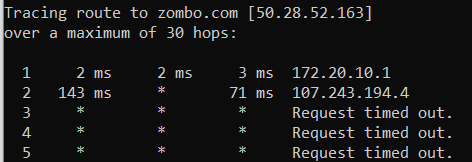
\includegraphics[width=\textwidth]{media/tracert_out.png}

\end{columns}

\end{frame}

\begin{frame}
\frametitle{Features}
\begin{itemize}
  \item RTT Analysis
  \item World Trace
  \item Long-term Comparisons
  \item Output Options
\end{itemize}
\end{frame}

\begin{frame}
\frametitle{RTT Analysis}

A descriptive statistical summary of the roundtrip times for 
a particular trace is output at the press of a button. Additionally,
the hop numbers on which packets were dropped are displayed.

\begin{center}
  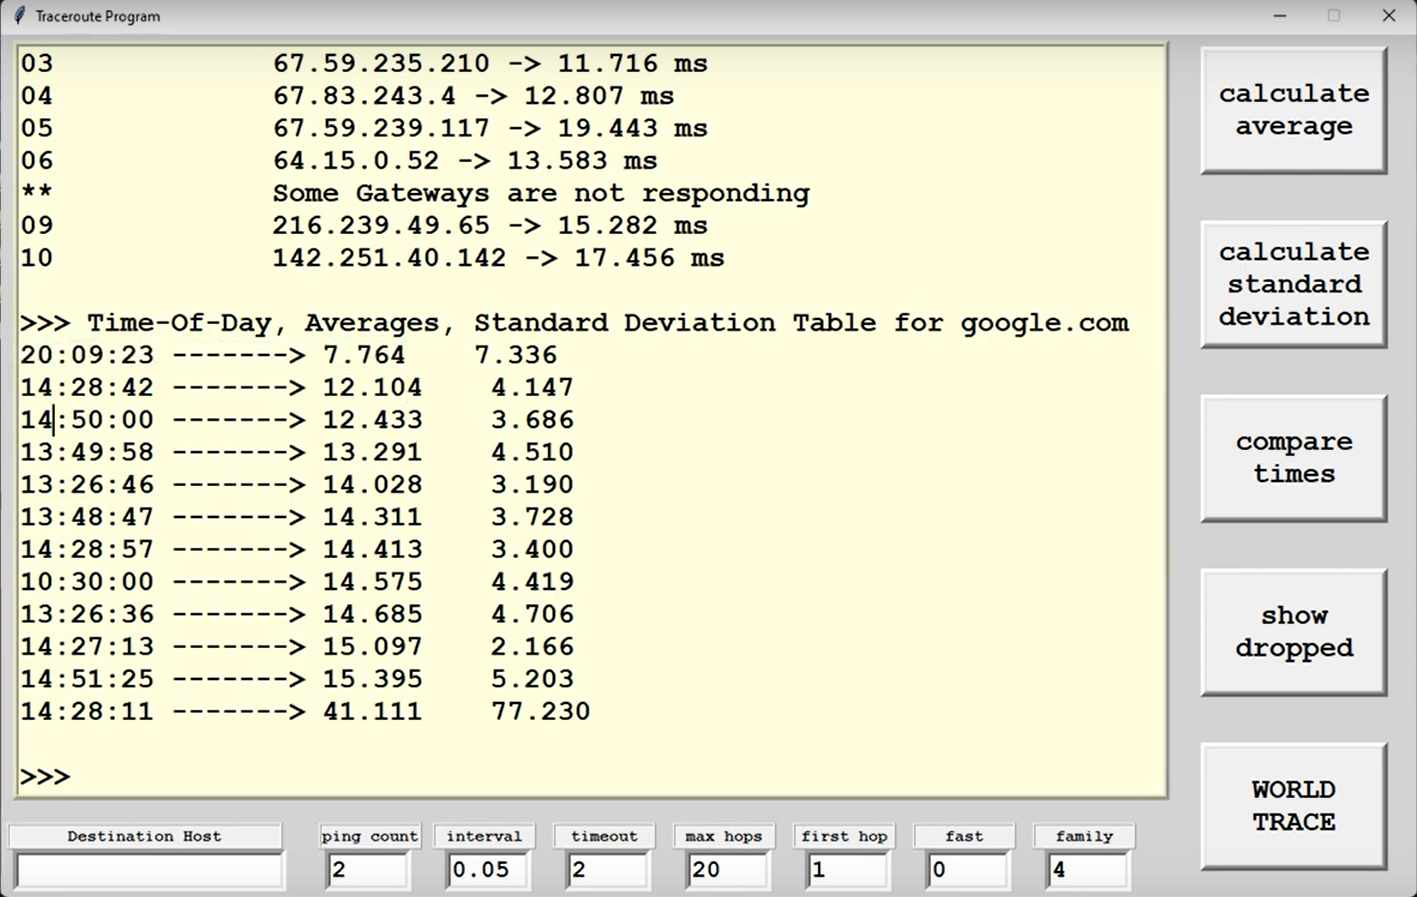
\includegraphics[width=0.6\textwidth]{media/stats.png}
\end{center}

\end{frame}

\begin{frame}
\frametitle{World Trace}

IPs visited during the trace are geolocated to form a map view of the 
path taken. As a result, users can look at the route from a geographical
perspective as opposed to the usual numeric outlook.

\begin{center}
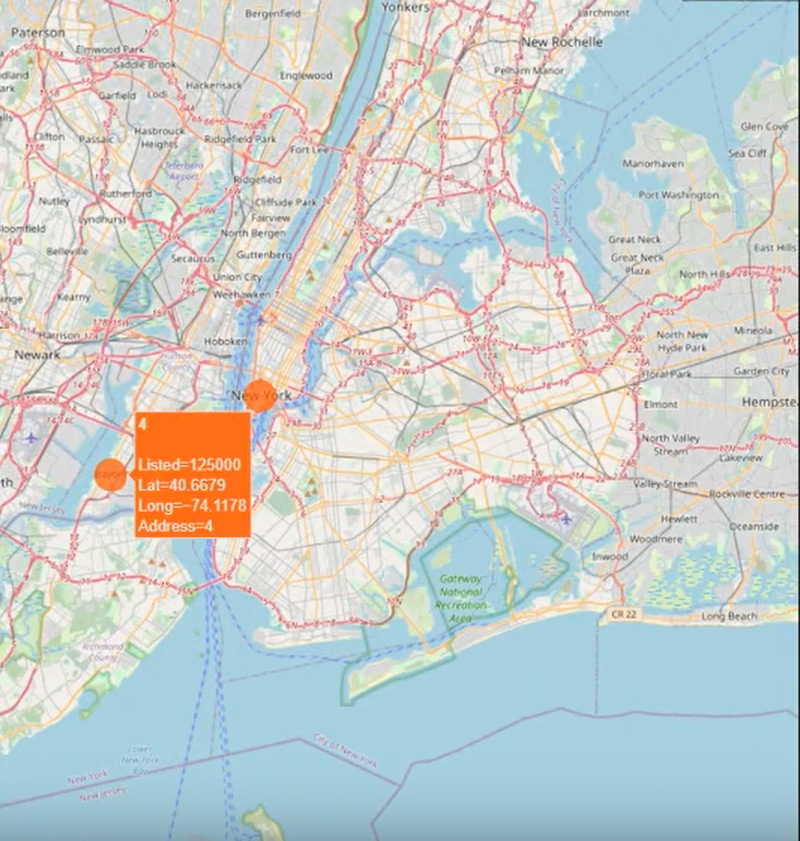
\includegraphics[width=0.4\textwidth]{media/worldtrace.png}
\end{center}

\end{frame}

\begin{frame}
\frametitle{Long-term Comparisons}

The updated traceroute program saves results for an IP each time a trace is performed.
With subsequent runs over time, the user can get an overview of how the stats of the 
trace change over a longer period.

% Since the packets may take varied paths throughout the day, storing data regarding
% the jumps to be compared later against previous runs will help analyze the health
% of the nodes along the typical path to a destination. 

\begin{center}
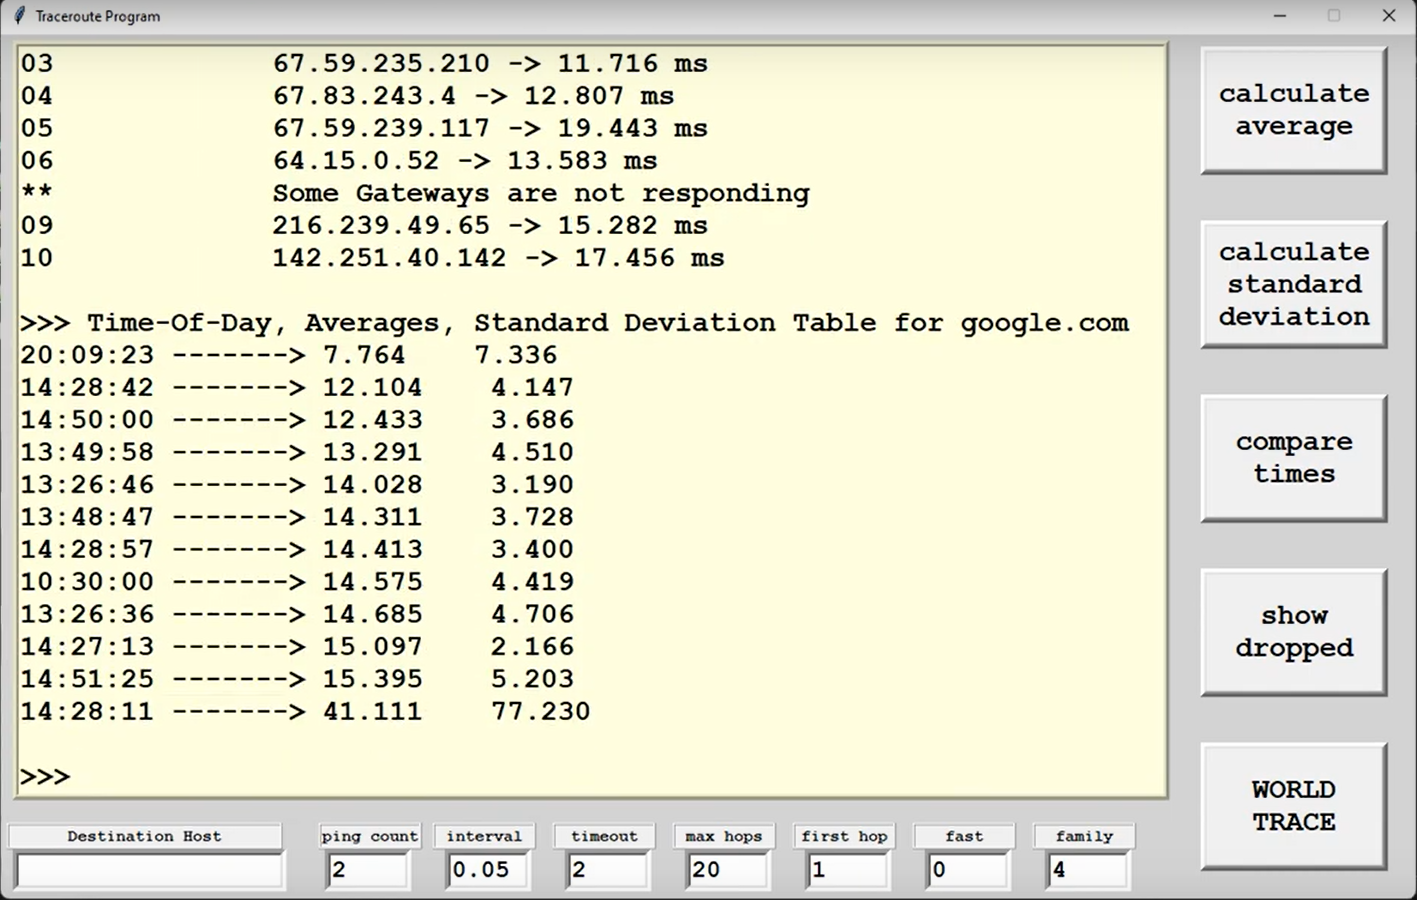
\includegraphics[width=0.6\textwidth]{media/compare.png}
\end{center}
\end{frame}

\begin{frame}

\frametitle{Output Options}

In case the user wishes to look deeper into the results of the traces,
information about the runs is saved in a \texttt{.csv} file, allowing
for deeper statistical analyses if desired. This is an improvement over 
the base \texttt{tracert} since the latter has no options to easily pipe
results into other programs.

\end{frame}

\begin{frame}
  \frametitle{Potential Directions Forward}

  \texttt{tracert} is already a minimal program, so core performance improvements
  are unlikely. However, any depth of statistic analysis could be implemented 
  from here on - the mean and standard deviation are only starting points.

  Additionally, more robust support for saving and analyzing old traces could be added.

  Finally, the web app currently used to display the World Trace could be moved
  to be part of the GUI.

\end{frame}

\begin{frame}
  \frametitle{Technologies Used}

\begin{itemize}
  \item \texttt{icmplib} - Python implementation of ICM protocol
  \item \texttt{tkinter} - GUI library
  \item \texttt{pandas} - quick statistical operations
  \item \texttt{requests} - used to convert IPs to locations
\end{itemize}

\end{frame}

\begin{frame}
  \frametitle{Links}

  \begin{itemize}
  \item \href{https://youtu.be/I2BpqN5PpAU}{\underline{GUI Traceroute Demo}}
  \item \href{http://github.com/mrinchanSIT/Traceroute}{\underline{\texttt{mrinchanSIT/Traceroute} on Github}}
  \end{itemize}
\end{frame}

\end{document}